\clearpage
\subsection{File Formats} % (fold)
\label{sub:file_formats}

There are two main file formats that you can work with in your program: binary files and text files. A text file stores its data as textual characters, whereas a binary file stores the values directly in the file. 

\begin{figure}[h]
   \centering
   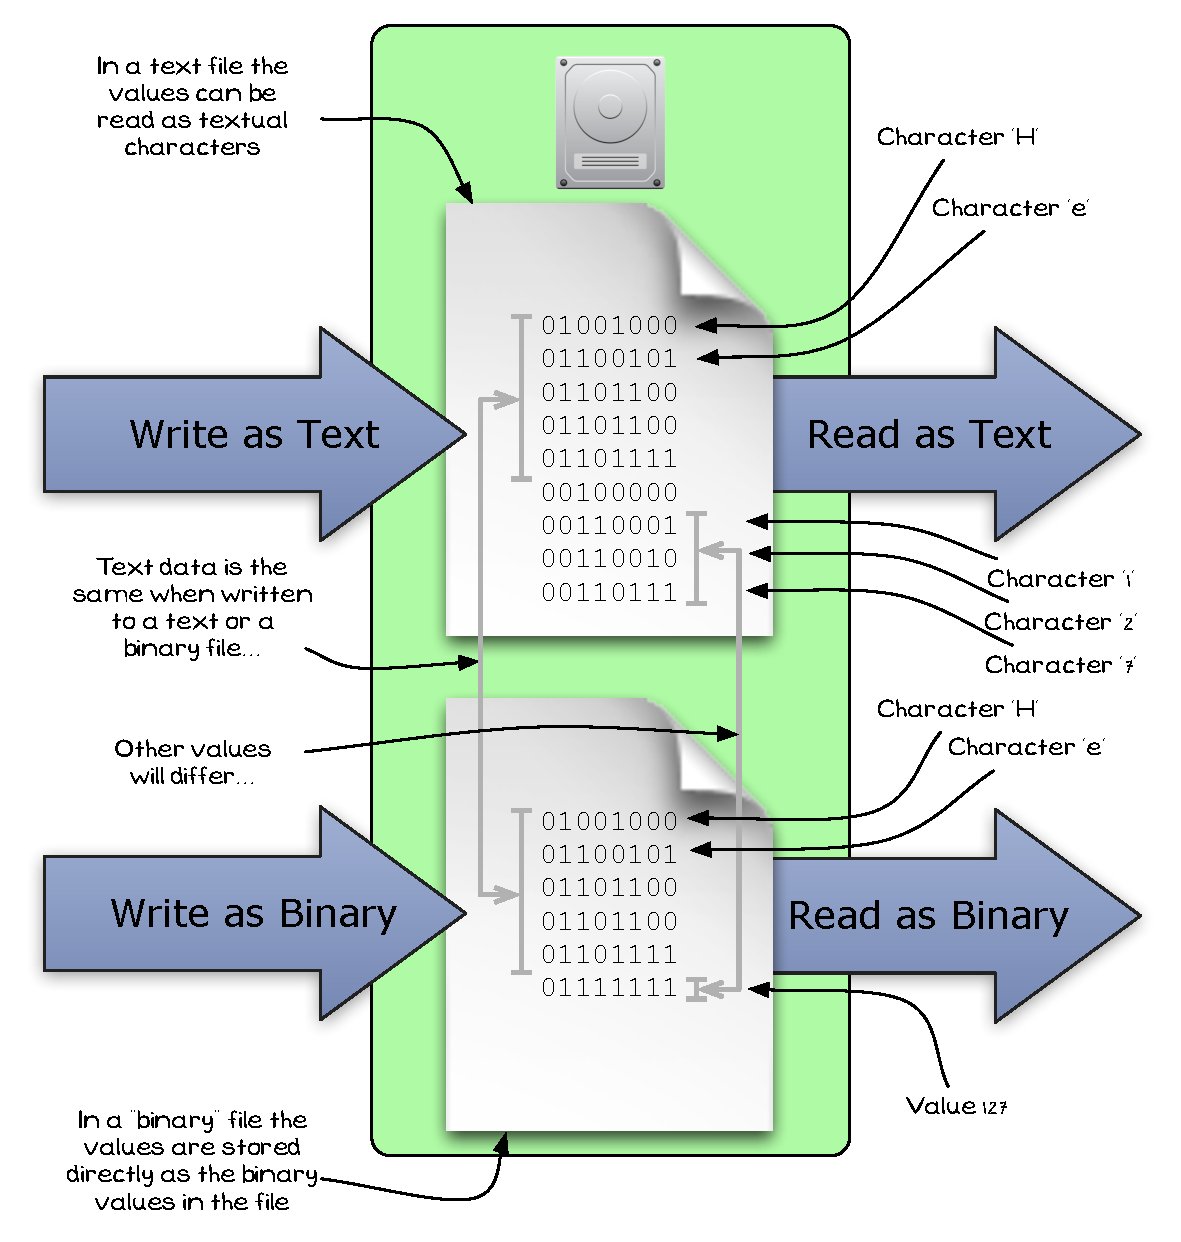
\includegraphics[width=0.9\textwidth]{./topics/file-io/diagrams/FileFormats} 
   \caption{Files can store \emph{textual} or binary data}
   \label{fig:file-formats}
\end{figure}

\mynote{
\begin{itemize}
  \item \fref{fig:file-formats} shows a binary and text file used to save the text `Hello' and the integer 127.
  \item In the \emph{text} file they are stored as the characters `H', `e', `l', `l', `o', and `1', `2', and `7' separated by a space.
  \item In the \emph{binary} file the characters are stored in the same way (as they are text), but the integer is stored as the value 127 which if interpreted as text is a \emph{delete} character.
  \item If you opened these files in a text editor you could read the values from the text file, but you would see a strange character instead of the number 127 in the binary file.
\end{itemize}
}


% subsection file_formats (end)